\documentclass[tikz, border=3mm]{standalone}
\usepackage{tikz}
\usetikzlibrary{arrows.meta, decorations.markings, calc} % Added calc library

\begin{document}
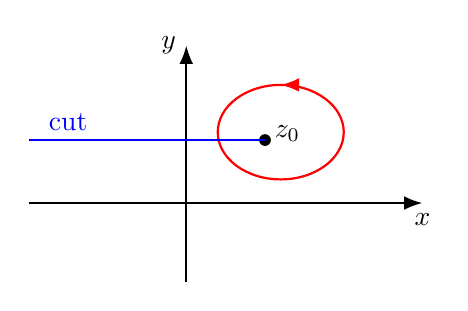
\begin{tikzpicture}[
    >=Latex, % Set default arrow tip style
    dot/.style={fill=black, circle, inner sep=1.5pt} % Style for points
]

% Axes
\draw[->, thick] (-2, 0) -- (3, 0) node[below] {$x$};
\draw[->, thick] (0, -1) -- (0, 2) node[left] {$y$};

% Define z0 coordinate
\coordinate (z0) at (1, 0.8);

% Draw the cut line extending left from z0
% Use the known y-coordinate of z0
\node[blue, above] at (-1.5, 0.8) {cut};

% Draw the point z0 and label it
\node[dot, label={[right]$z_0$}] at (z0) {};

% Draw the red closed curve (ellipse) around z0
% Center the ellipse slightly offset from z0 for visual appearance
\draw[red, thick,
    postaction={decorate, decoration={markings, mark=at position 0.25 with {\arrow{>}}}} % Counter-clockwise arrow near top
] ($(z0)+(0.2,0.1)$) ellipse (0.8 and 0.6); % Adjust offset and radii as needed

\draw[blue, thick] (-2, 0.8) -- (z0);

\end{tikzpicture}
\end{document}